\chapter{Schramm-Loewner Evolutions}
\label{ch4-sle}

Lorem ipsum dolor sit amet, consectetur adipisicing elit, sed do eiusmod tempor
incididunt ut labore et dolore magna aliqua. Ut enim ad minim veniam, quis
nostrud exercitation ullamco laboris nisi ut aliquip ex ea commodo consequat.
Duis aute irure dolor in reprehenderit in voluptate velit esse cillum dolore eu
fugiat nulla pariatur. Excepteur sint occaecat cupidatat non proident, sunt in
culpa qui officia deserunt mollit anim id est laborum.

\begin{equation}
    \partial_t g_t(z) = \frac{2}{g_t(z) - U_t}
    \label{eq:loew}
\end{equation}

\section{Loewner Evolutions}
\label{sec:le}

\section{Stochastic Loewner Evolutions}
\label{sec:le}

\textbf{Coformal Invariance.}
We talked extensively in Chapter~\ref{ch3-conf} about conformal invariance and
its importance to the study of critical systems. There we used a field
theoretical approach, but in the context of measure theory, conformal
invariance is stated as
\begin{equation}
    \newcommand{\pp}[1]{\left(#1\right)}
    f\circ\mu_D\pp{z,w} = \mu_{f(D)}\pp{f\pp{z}, f\pp{w}}.
\end{equation}
This is to say, given a domain $D$ and a set of curves $\gamma$ that connect
the points $z$ and $w\in\partial D$, the measure $\mu$ of this family of curves
is invariant under a conformal transformation $f$. In simpler words, it means
that if you have a certain (continuum) model $M$ and use it to generate a set
of curves in $D$ and then conformally map the curves to $f(D)$, these
curves would have the same statistical properties as if you simply generated the
curves by applying $M$ to $f(D)$ directly. An illustration can be seen in
Figure~\ref{fig:confinv}.


\textbf{Domain Markov Property.}
In his work, Schramm identified another fundamental property that conformally
invariant lattice models tend to obbey called domain Markov property. It
stated as
\begin{equation}
    \newcommand{\pp}[1]{\left(#1\right)}
    \mu_D\pp{\gamma_2|\gamma_1} = \mu_{D\setminus\gamma_1}\pp{\gamma_2}.
\end{equation}
That is, the conditional measure of family of curves $\gamma_2$ that have the
same start $\gamma_1$ in a domain $D$ is the same as that of $\gamma_2$ in
a domain with $\gamma_1$ removed, that is, $D\setminus\gamma_1$.
In the same line of conformal invariance, domain Markov property can be
understood in the following way: if you have a model M and use it to generate a
set of curves in $D$ that all have the same start $\gamma_0$, the curves
$\gamma_1$ obtained would have the exact same properties as if you generated
the curves by applying M to $D\setminus\gamma_0$. An illustration can be
seen in Figure~\ref{fig:dmp}.

\begin{figure}
\begin{center}
    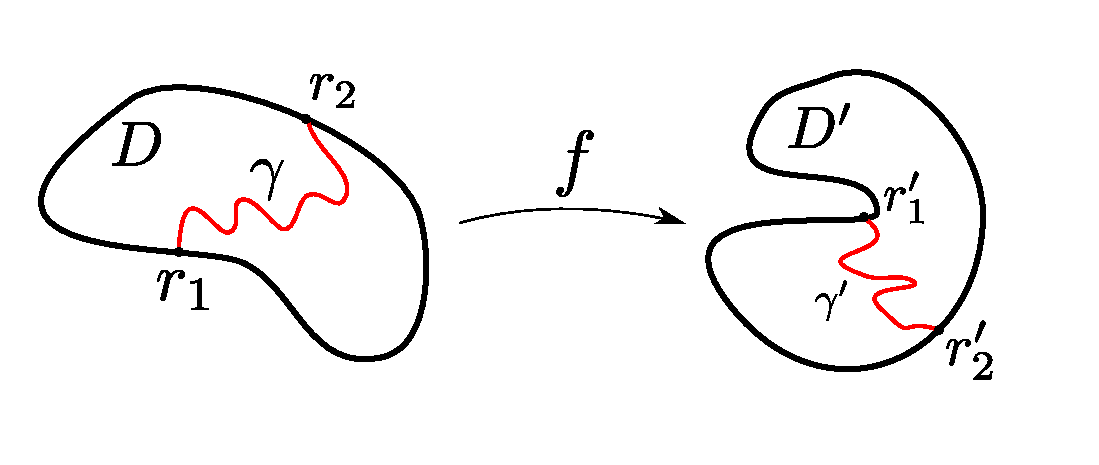
\includegraphics[scale=0.8]{chapters/ch4-sle/figs/confinv}
\end{center}
\caption{Lorem ipsum dolor sit amet, consectetur adipisicing elit, sed do
    eiusmod tempor incididunt ut labore et dolore magna aliqua. Ut enim ad
    minim veniam, quis nostrud exercitation ullamco laboris nisi ut aliquip ex
    ea commodo consequat. Duis aute irure dolor in reprehenderit in voluptate
    velit esse cillum dolore eu fugiat nulla pariatur. Excepteur sint occaecat
    cupidatat non proident, sunt in culpa qui officia deserunt mollit anim id
    est laborum.}
\label{fig:confinv}
\end{figure}


\begin{figure}
\begin{center}
    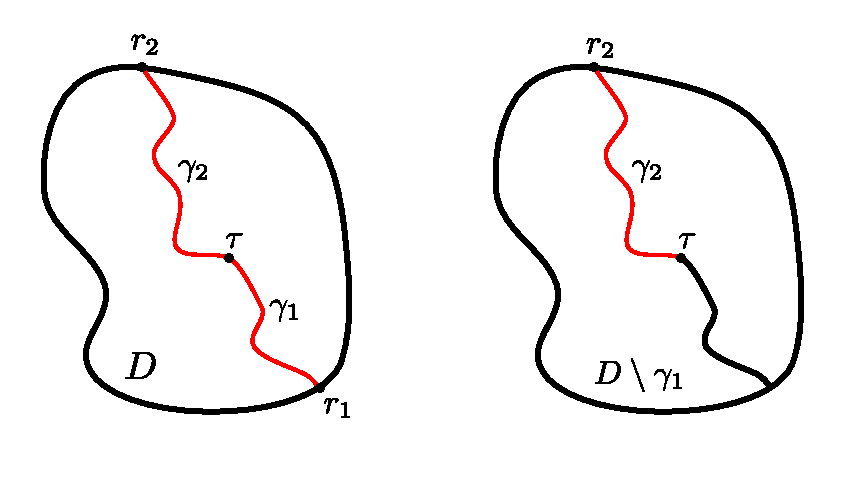
\includegraphics[scale=0.9]{chapters/ch4-sle/figs/dmp}
\end{center}
\caption{The domain Markov property states that the conditional measure of
    $\gamma_2$ given a fixed $\gamma_1$ in a domain $D$ is the same of $\gamma_2$
    in the same domain with $\gamma_1$ removed, that is, $D\setminus\gamma_1$.}
\label{fig:dmp}
\end{figure}


\section{Numerical Methods}
\label{sec:num}

The crux of the Schramm Loewner Evolution problem is determining whether or not
a given model converges to it in the continuum limit, and what is the value of
$\kappa$ for this specific model. We mentioned several models that have been
proven to asdasd, the most illustrious being Smirnov's demonstration that
percolation in a triangular lattice converges to SLE with $\kappa=6$.

Nonetheless, just like nobody would expect every critical system to have an
exact solution similar to the Ising model, one may not expect to be able to
prove the SLE convergence for every conceivable model. To be completely
fair, we cannot there is no way to know this prove is impossible either, but

This is where
numerical analysis comes into the scene. By comparing the statistical behavior
of the model with the expected SLE trace, we can infer Eq.~\ref{eq:prob} holds
true.

\subsection{Euler's Method}
\label{ss:euler}

Euler's method for solving ordinary differential equations is arguably the
simplest. It is used to solve equation of the type $y'(t) = f(y, t)$ and it
basically consists in taking a first order approximation of the solution
\begin{equation}
    \newcommand{\y}[1]{y\left(#1\right)}
    \newcommand{\f}[1]{f\left(#1\right)}
    \y{t} = \y{t_0} + \int_{t_0}^t \f{\y{\tau}, \tau} d\tau \approx
            \y{t_0} + \left(t - t_0\right)\f{\y{t_0}, t_0}.
\end{equation}
This way, the equation can be solved recursivelly by providing a discretized
driving function $U_{t_i}$ with $t_0 = 0 < t_{1}<\cdots<t_N$ and. Applying it
to Loewner's equation (Eq.~\ref{eq:loew}) we have
\begin{equation}
    g_{t_{i+1}}(z) = g_{t_i}(z) + (t_{i+1} - t_i) \frac{2}{g_t(z) - U_{t_i}}.
\end{equation}

In order to obtain the trace from $g_t$ we take the fact that
\begin{equation}
    g_t(\gamma_t) = U_t.
    \label{eq:root}
\end{equation}
You can use your favorite method of root finding to solve Eq.~\ref{eq:root} for
$\gamma_t$. In Figure~\ref{fig:euler1} you can see a realization for
$\kappa=2$. In it we colored the grid according to the sign of
$Re\{g_t(z)-U_t\}$. The border between the positive and negative sides should
be around the region where the trace is. We also observe the most blatant
drawback of the method: it fails in several points, where they get mapped
outside the upper half plane, which is not allowed in chordal Loewner's
evolutions. This problem accentuates quickly as the value of $\kappa$ rises,
to the point where the case $\kappa=6$ (Figure~\ref{fig:euler2}) has barely
any discernible trace.

Other problem with Euler's method in the context of Loewner evolutions is
computational complexity. It requires $O(N)$ for each point of the space where
you compute $g_t(z)$, considering the you use a $(M,M)$ regular grid, the whole
algorithm have complexity $O(NM^2)$. This is further aggravated by the fact the
most points are not necessary to actually compute the trace, making most of the
computational effort useless. One possible advantage is the fact that this
algorithm is highly parallelizable, although this is hardly an advantage faced
with the other drawbacks.

\begin{figure}
\begin{center}
    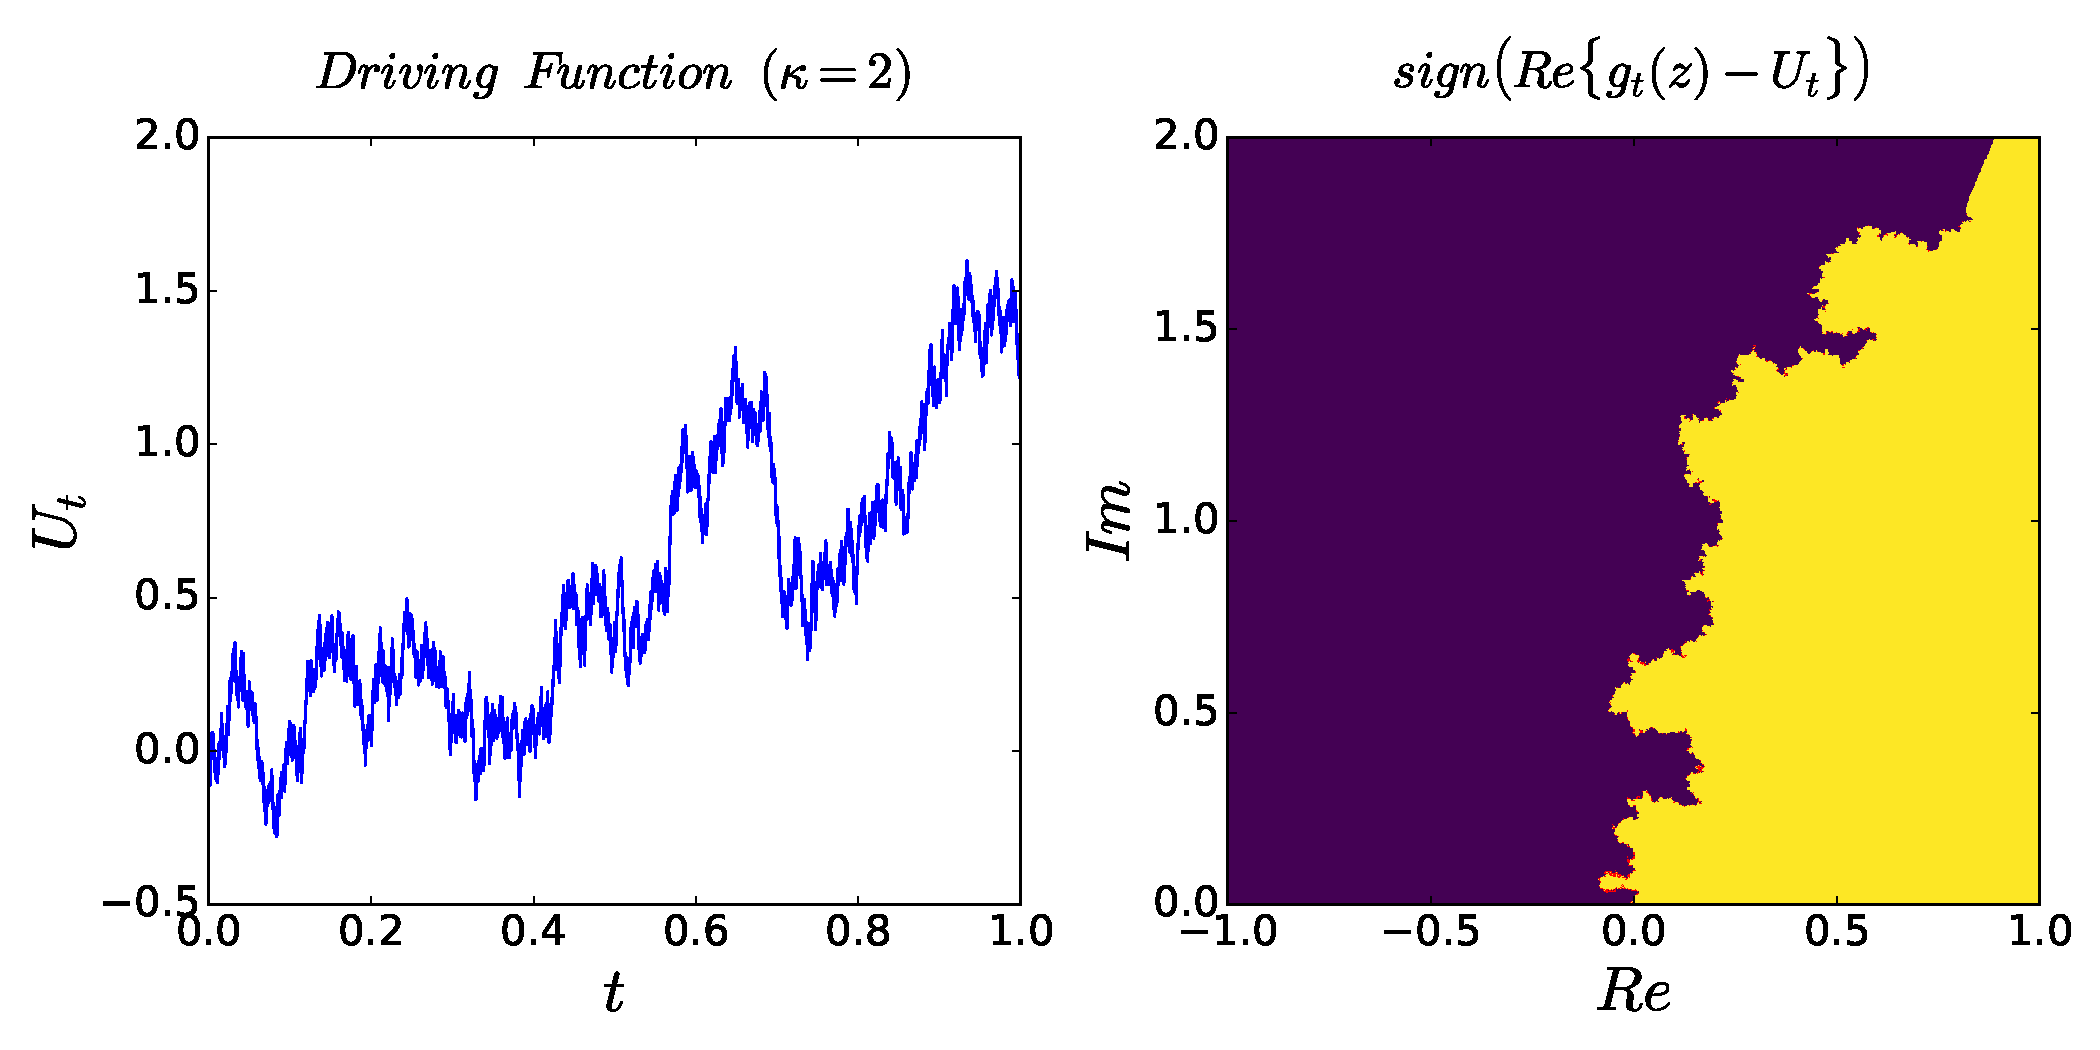
\includegraphics[scale=0.45]{chapters/ch4-sle/figs/euler1}
\end{center}
\caption{Simulation of an SLE process with $\kappa=2$ using the Euler method
    with $\Delta t = 10^{-5}$ in a grid of resolution $(1024, 1024)$. Because
    at time $t$ $g_t(\gamma_t)-U_t=0$, if we color the upper half plane
    according to which side of the real line each point is mapped, the border
    between the regions should indicate the position of the trace $\gamma_t$.
    The red points are the points where the method failed and were mapped
    outside the upper half plane. The smooth ``tail'' of the trace happens
    because these points have not yet been mapped to the real line.}
\label{fig:euler1}
\end{figure}

\begin{figure}
\begin{center}
    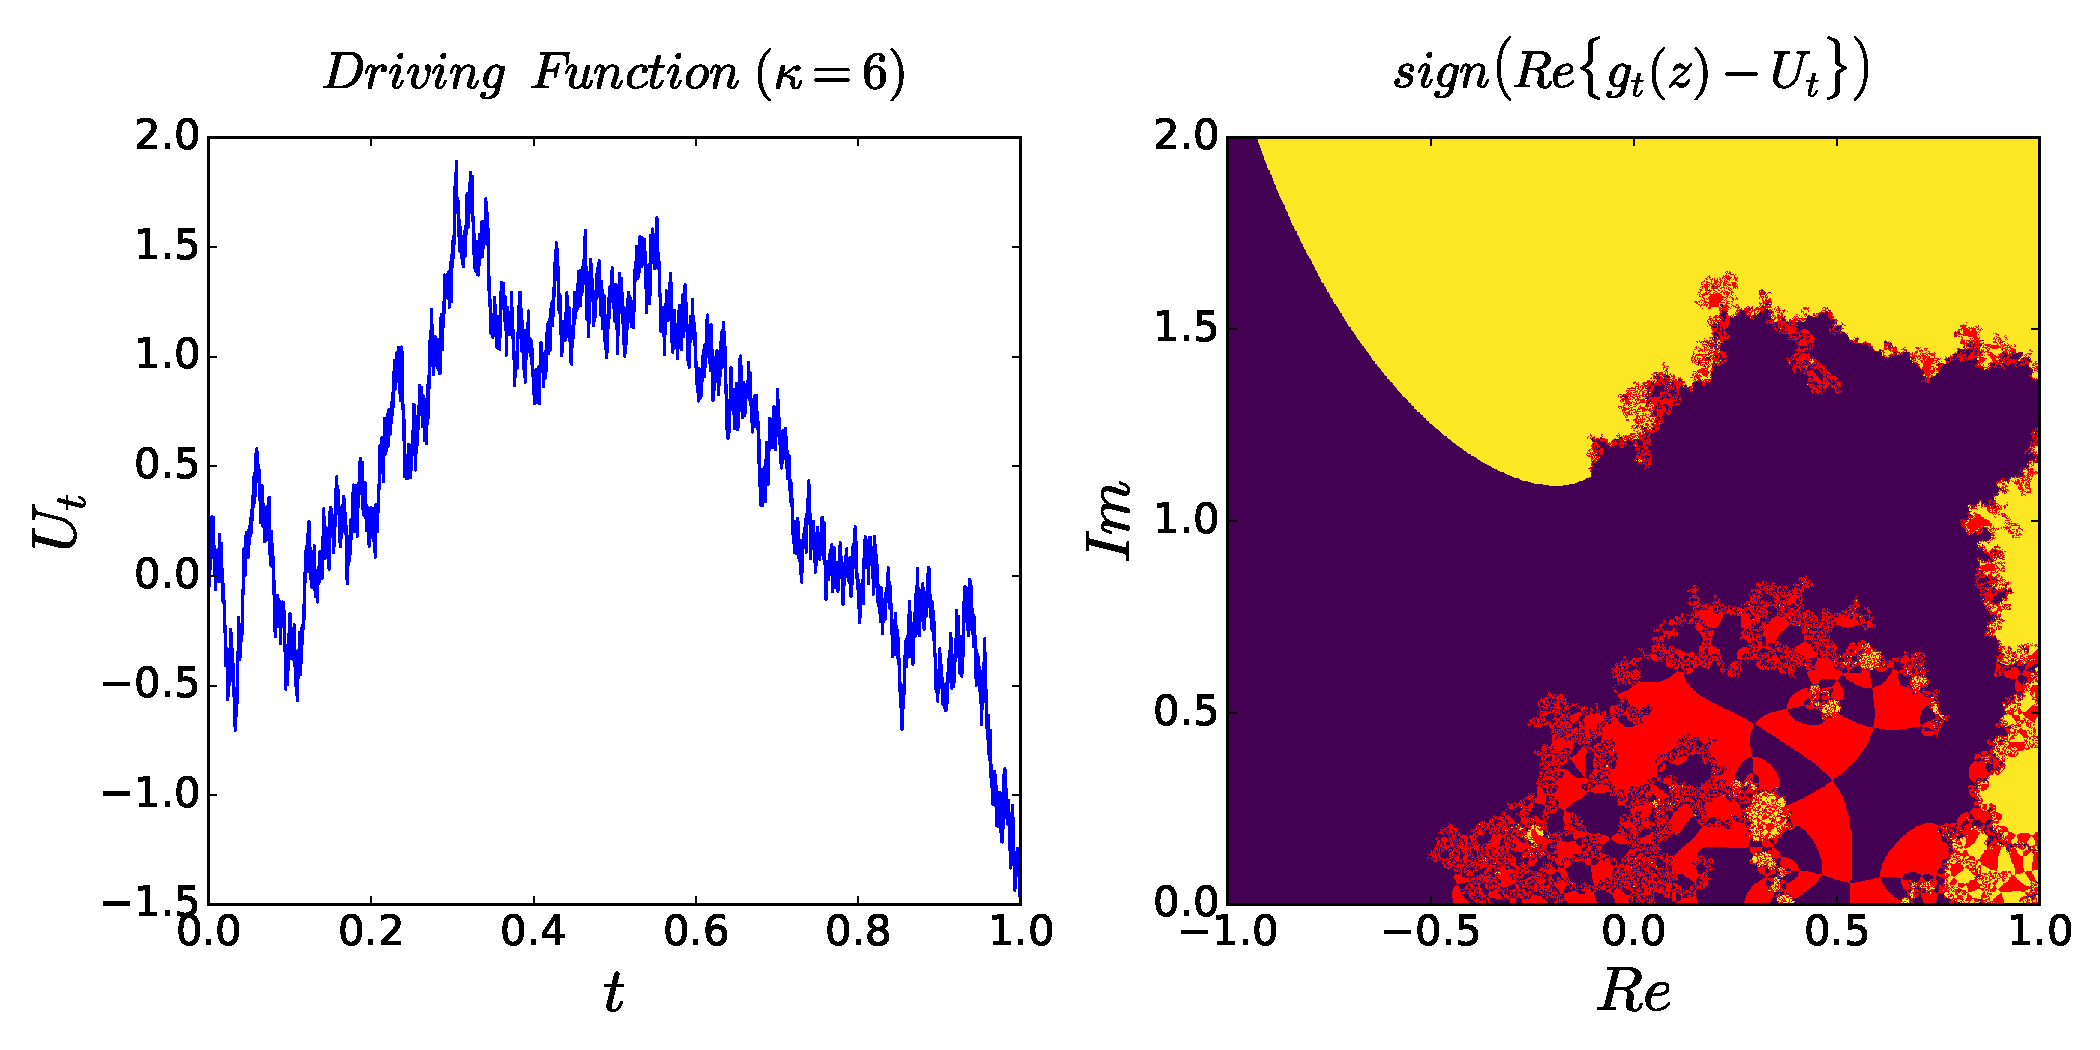
\includegraphics[scale=0.45]{chapters/ch4-sle/figs/euler2}
\end{center}
\caption{Simulation of an SLE process with $\kappa=6$ using the Euler method
    with $\Delta t = 10^{-5}$ in a grid of resolution $(1024, 1024)$. 
    The red points are the points where the method failed and were mapped
    outside the upper half plane. The algorithm performed much worse than
    the case $\kappa=2$.}
\label{fig:euler2}
\end{figure}


\subsection{Zipper Algorithm}
\label{ss:zipper}

Let $0<s<t$. The map $g_{s+t}$ takes $\HH\setminus\gamma_{[0,s+t]}$ to $\HH$.
If we try to do it in two steps, we may take $g_s$ to map 
$\HH\setminus\gamma_{[0,s]}$ to $\HH\setminus\gamma_{[s, s+t]}$ and 
$\bar{g}_{t}$ to map $\HH\setminus\gamma_{[s, s+t]}$ to $\HH$. The
map $\bar{g}_t$ is evidently not the same as $g_t$, but the 
$\bar{g}_t(z-U_s)+U_t$ 

\begin{figure}
\begin{center}
    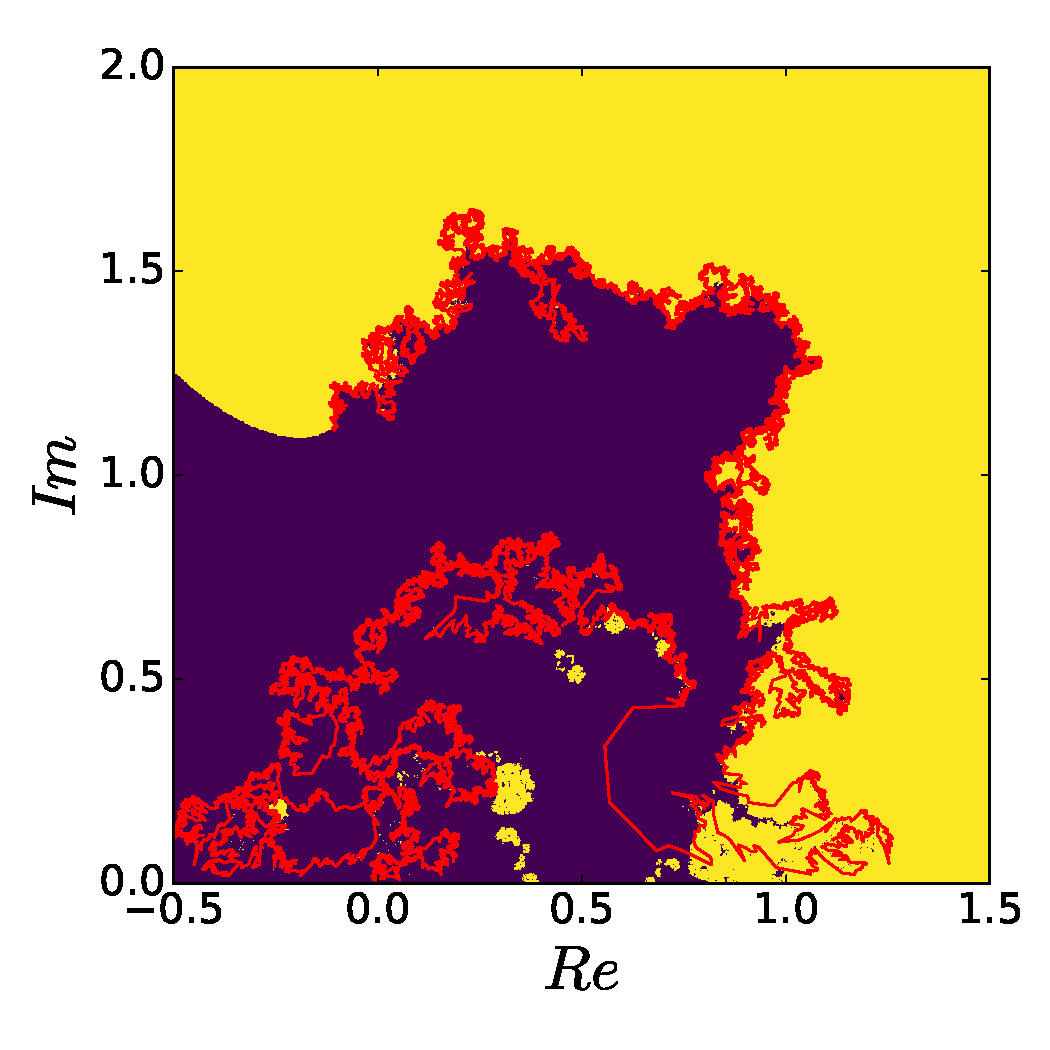
\includegraphics[scale=0.5]{chapters/ch4-sle/figs/eulerzip}
\end{center}
\caption{Comparison of the traces obtained by using the zipper algorithm (red
    line) and Euler's method. Although it presents large jumps in the trace due
    to large displacements in the driving function, zipper it still performs
    better than the Euler's.}
\label{fig:euzip}
\end{figure}

\begin{figure}
\begin{center}
    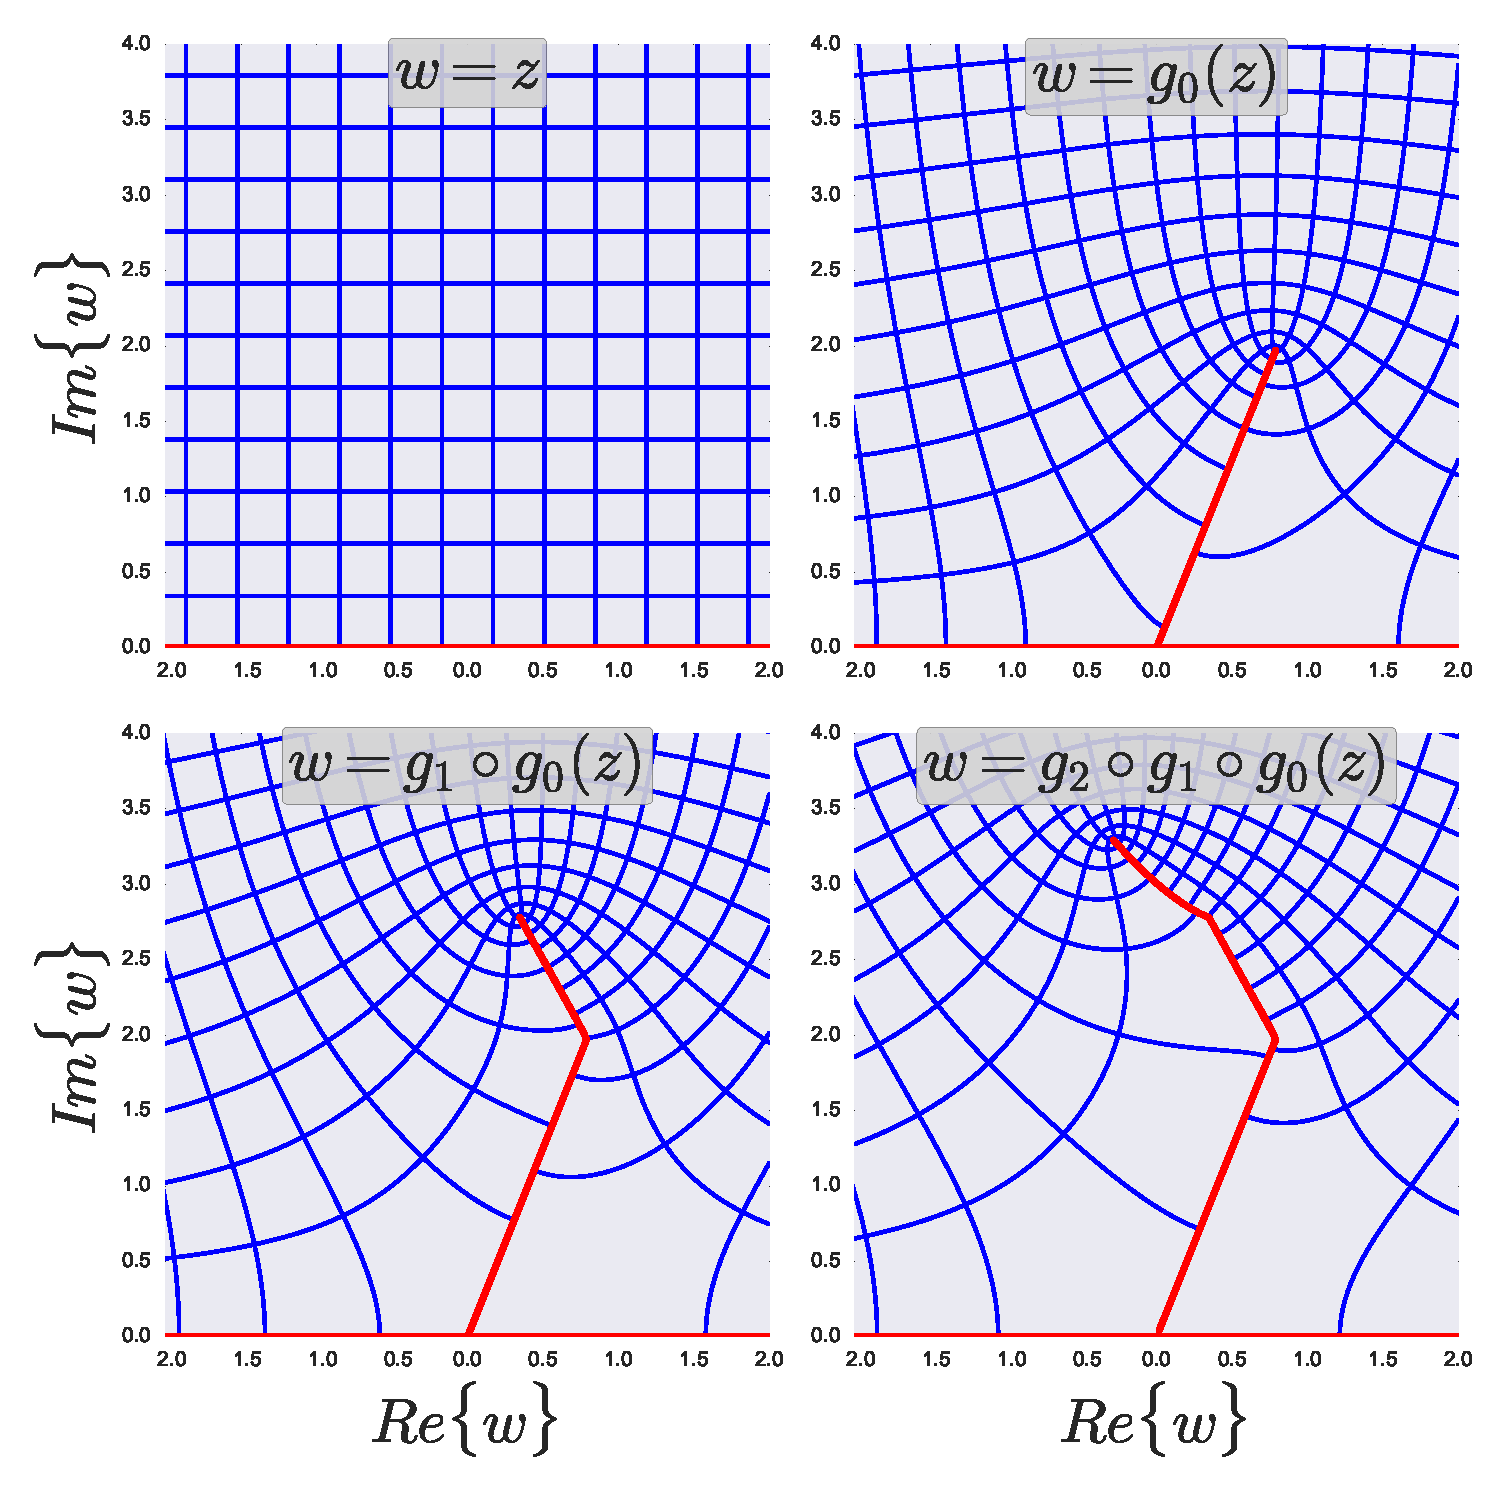
\includegraphics[scale=0.5]{chapters/ch4-sle/figs/zipper}
\end{center}
\caption{Result of applying the first three iterations of the zipper algorithm
    with the tilted slit approximation. In the limit $\Delta t\rightarrow 0$
    the red line converges to an SLE trace.}
\label{fig:zipper}
\end{figure}
